\documentclass[,a4paper,12pt]{article}
\usepackage[utf8]{inputenc}
\usepackage[siunitx]{circuitikz}
\usepackage{graphicx}
\usepackage{multirow}
\usepackage{float}
\usepackage{makecell} % Pakiet do łamania wierszy w tabeli
\usepackage[table]{xcolor}
\usepackage{cellspace}
\setlength{\cellspacetoplimit}{4pt} % Górny padding
\setlength{\cellspacebottomlimit}{4pt} % Dolny padding
\usepackage{array}
\usepackage{amsmath}
% Odstępy w tabelach
\setlength{\tabcolsep}{8pt} % Poziome odstępy
\renewcommand{\arraystretch}{1.5} % Pionowe odstępy
\newenvironment{conditions}
  {\par\vspace{\abovedisplayskip}\noindent\begin{tabular}{>{$}l<{$} @{${}={}$} l}}
  {\end{tabular}\par\vspace{\belowdisplayskip}}
\usepackage[T1]{fontenc}
\usepackage[MEX]{polski}
\usepackage{booktabs}
\usepackage[usenames,dvipsnames]{xcolor}
\usepackage{geometry}
\usepackage{siunitx} % Dodanie pakietu siunitx do formatowania jednostek
\sisetup{separate-uncertainty, output-decimal-marker = {,}}
\geometry{a4paper, total={170mm,257mm}, left=20mm, top=20mm}
\usepackage{indentfirst} % Dodaje wcięcia po sekcjach
\setlength{\parindent}{1em} % Ustawia globalne wcięcia w akapitach
\renewcommand{\footnotesize}{\fontsize{10pt}{12pt}}
%\renewcommand{\thesection}{\Roman{section}}
\usepackage[backend=biber,style=numeric, sorting=none]{biblatex}
\addbibresource{bibliografia.bib} % Wskaż plik .bib z wpisami bibliograficznymi
\usepackage{biblatex}
\renewcommand{\cite}{\supercite}
\usepackage{titlesec}
\titlespacing*{\paragraph}{0pt}{1.5ex plus 1ex minus .2ex}{1.5ex plus 1ex minus .2ex}
\titleformat{\paragraph}[block]{\normalfont\normalsize\bfseries}{\theparagraph}{1em}{}
\usepackage[pdfusetitle]{hyperref}
\hypersetup{
    pdfauthor={Inez Małecka},
    pdftitle={Sprawozdanie laboratoryjne}, 
    pdfsubject={Praca wykonana samodzielnie, jestem jedynym autorem.}, 
    pdfkeywords={potencjometr, prawo Ohma, raport, laboratorium}, 
}



\begin{document}
\begin{center}
    \begin{tabular}{|p{6cm}|p{4.5cm}|p{4.5cm}|}
        \hline
        \multicolumn{3}{|c|}{\textbf{\large ELEKTRONIKA I ELEKTROTECHNIKA}} \\ 

        \multicolumn{3}{|c|}{\textbf{ Laboratorium}} \\
        \hline
        \multicolumn{3}{|l|}{Temat ćwiczenia: Układy cyfrowe - podstawowe bramki logiczne} \\
        \hline
        {\small Ćwiczenie wykonała:} &
        {\small Numer ćwiczenia:} &
        {\small Prowadzący:} \\
        \begin{center}
            \textbf{Inez Małecka (52738) }
        \end{center} &
        \begin{center}
            \textbf{Lab09}
        \end{center} &
        \begin{center}
            \textbf{Mgr inż. Leszek Kędzierski}
        \end{center}
        \\
        \hline
        {\small Sprawozdanie opracowała:} &
        {\small Data wykonania ćwiczenia:} &
        {\small Ocena:} \\
        \begin{center}
            \textbf{
        Inez Małecka (52738)}
        \end{center}
         &
         \begin{center}
             \textbf{20/01/2025}
         \end{center}
        &
        \\
        \hline
    \end{tabular}
\end{center}
\section{{\textsc{Wprowadzenie}}}
Celem niniejszego ćwiczenia było zapoznanie się z działaniem oraz zasadami działania podstawowych układów cyfrowych - bramek logicznych. W trakcie wykonywania powyższego zadania domowego szczególną uwagę poświęcono zrozumieniu działania podstaw jakimi kierują się bramki logiczne, oraz analizie ich możliwych kombinacji. \\\par
Algebra Boole'a jest strukturą matematyczną postaci :\cite{ligeza_elementy_logiki}
\begin{equation}
    (\{0,1\},\vee,\wedge,\neg,0,1)
\end{equation}
Określana inaczej jako algebra zero-jedynkowa opisuje działania logiczne gdzie dany zbiór dwuelementowy, działania alternatywy, koniunkcji, negacji, sumy i iloczynu tworzą kratę (zbiór częściowo uporządkowany gdzie kresem górnym jest $1$, a kresem dolnym jest $0$). Krata dystrybucyjna ze względnymi dopełnieniami określana inaczej jako kratą boolowską, w takiej kracie obowiązują prawa dzięki którym określenie jest struktury, dopełnień i możliwych koniugacji jest matematycznie możliwe, a przeniesienie logiki Boole'a do rzeczywistości pozwala na fizyczne wykorzystanie logiki matematycznej w operacjach logicznych.\cite{Zynel2009} \\ \par
Działania algebry Boole'a spełniają następujące prawa:
\begin{itemize}
    \item Element neutralny - obecność wartości neutralnej nie wpływa na wynik działania, co pozwala zachować spójność elementów.
    \item Identyczność - wykorzystanie stałych $(0\hspace{5pt}lub\hspace{5pt}1)$ w wyrażeniu przesądza o jego wyniku,
    \item Idempotentność - wielokrotne zastosowanie tej samej operacji do elementu nie wprowadza nowych elementów, 
    \item Dopełnienie - każdy element posiada swoją negację,
    \item Przemienność - składniki można dowolnie zamieniać miejscami,
    \item Łączność - sposób grupowania można zmieniać bez wpływu na wynik,
    \item Rozdzielność - $\vee \hspace{5pt}oraz\hspace{5pt}\wedge$ rozkładają się wzajemnie na siebie analogicznie jak w zwykłej algebrze,
    \item Pochłanianie - pewne wyrażenia logiczne można sprowadzić do prostej postaci poprzez pochłodnienie logicznie słabszego wyrażenia, 
    \item Prawo De Morgana - negacja koniunkcji przekłada się na alternatywę negacji, 
\end{itemize} \\ \par
W szerszym ujęciu, algebra Boole'a, w której opisano powyższe prawa, stanowi bazę teoretyczną do analizy i syntezy układów cyfrowych. Każde wyrażenie booleowskie (np.~reprezentujące sumę lub iloczyn logiczny zmiennych) można odwzorować w postaci bramek logicznych, stanowiących fizyczną implementację operacji \(\land\), \(\lor\) oraz \(\neg\). Dzięki temu możliwe jest tworzenie układów kombinacyjnych, przetwarzających sygnały zero-jedynkowe zgodnie z regułami opisanymi w algebrze Boole'a, jak również układów sekwencyjnych, jeśli do ich struktury wprowadzi się pętle sprzężenia zwrotnego (na przykład w postaci par bramek NAND lub NOR, tworzących przerzutniki).\cite{CEAutomatyki}

Istotne znaczenie w projektowaniu i analizie układów cyfrowych mają tzw.\ systemy funkcjonalnie pełne, dzięki którym każdą funkcję booleowską można zrealizować, dysponując tylko jednym rodzajem bramek. Klasycznymi przykładami są bramki NAND (kreska Sheffera) i NOR (strzałka Peirce’a), nazywane bramkami uniwersalnymi. W dowolnej liczbie oraz konfiguracji pozwalają one na skonstruowanie wszelkich innych bramek (AND, OR, NOT, XOR) i funkcji logicznych, zapewniając niezwykłą elastyczność podczas projektowania sprzętu oraz możliwość standaryzacji procesu produkcji.\cite{WikipediaFunctionalCompleteness} Wszystkie opisane własności algebry Boole'a, jak również zestaw bramek logicznych realizujących jej operacje, tworzą fundament inżynierski wykorzystywany zarówno w prostych układach realizujących podstawowe zadania logiczne, jak i w skomplikowanych procesorach, układach ASIC czy programowalnych strukturach FPGA, które operują na tysiącach lub milionach kombinacji sygnałów cyfrowych jednocześnie.\cite{WikipediaLogicGate}

\section{\textsc{Przebieg zadania}}
\subsection{\textsc{Symulacja podstawowych układów logicznych}}
Zadanie wykonano przy pomocy materiałów edukacyjnych znajdujących się na platformie \texttt{moodle2.e-wsb.pl/} oraz darmowej wersji symulatora podstawowych układów logicznych - \texttt{logic.ly/}. \\ \par
W celu poprawnego zapoznania się z działaniem bramek logicznych, przeprowadzono symulację działania najpopularniejszych bramek logicznych oraz zapisano wyniki symulacji w formie tabeli dla każdej z nich:
\begin{itemize}
    \item \paragraph{\textsc{Bramka logiczna \textit{NOT}}}
    \begin{minipage}{0.45\textwidth}
    \centering
    % Tabela prawdy
    \begin{tabular}{c|c}
        $X_1$  & $Y$ \\ \hline
        1 & 0 \\ 
        0 & 1 \\ 
    \end{tabular}
\end{minipage}
\hfil
\begin{minipage}{0.45\textwidth}
    \centering
    % Schemat bramki logicznej
    \begin{circuitikz}
    % Wejście X1
    \node (A) at (0,0) {$X_1$}; % Węzeł wejścia
    % Bramkę NOT ustawiamy w odpowiednim miejscu
    \node [not port, anchor=in] (NOT) at (1.5,0) {}; % Bramkę NOT umieszczamy
    % Wyjście
    \node (OUT) at (4,0) {$Y$}; % Węzeł wyjścia
    % Łączymy elementy
    \draw (A) -- (NOT.in); % Połączenie wejścia z bramką
    \draw (NOT.out) -- (OUT); % Połączenie bramki z wyjściem
    \end{circuitikz}
\end{minipage}
\item \paragraph{\textsc{Bramka logiczna \textit{AND}}}
\begin{minipage}{0.45\textwidth}
    \centering
    % Tabela prawdy
    \begin{tabular}{c|c|c}
        $X_1$ & $X_2$ & $Y$ \\ \hline
        1 & 1 & 1 \\ 
        1 & 0 & 0 \\
        0 & 1 & 0 \\
        0 & 0 & 0 \\
    \end{tabular}
\end{minipage}
\hfil
\begin{minipage}{0.45\textwidth}
    \centering
    % Schemat bramki logicznej
    \begin{circuitikz}
    % Punkt referencyjny dla wejścia X1
    \node (A) at (0,1) {$X_1$}; % Węzeł wejścia 1 (górny)
    % Punkt referencyjny dla wejścia X2
    \node (B) at (0,-1) {$X_2$}; % Węzeł wejścia 2 (dolny)

    % Bramkę AND ustawiamy dokładnie na środku pomiędzy A i B
    \node[and port, anchor=center] (AND) at (3,0) {}; % Bramkę ustawiamy centralnie

    % Wyjście bramki ustawione w jednej linii z jej środkiem
    \node (OUT) at (4,0) {$Y$}; % Węzeł wyjścia

    % Łączenie wejść z bramką AND
    \draw (A.east) -- (AND.in 1); % Połączenie wejścia X_1 z górnym portem bramki
    \draw (B.east) -- (AND.in 2); % Połączenie wejścia X_2 z dolnym portem bramki
    
    % Łączenie wyjścia bramki z punktem OUT
    \draw (AND.out) -- (OUT.west); % Połączenie wyjścia bramki z OUT
\end{circuitikz}

\end{minipage}
\item \paragraph{\textsc{Bramka logiczna \textit{NAND}}}
\begin{minipage}{0.45\textwidth}
    \centering
    % Tabela prawdy
    \begin{tabular}{c|c|c}
        $X_1$ & $X_2$ & $Y$ \\ \hline
        1 & 1 & 0 \\ 
        1 & 0 & 1 \\
        0 & 1 & 1 \\
        0 & 0 & 1 \\
    \end{tabular}
\end{minipage}
\hfil
\begin{minipage}{0.45\textwidth}
    \centering
    % Schemat bramki logicznej
    \begin{circuitikz}
    % Punkt referencyjny dla wejścia X1
    \node (A) at (0,1) {$X_1$}; % Węzeł wejścia 1 (górny)
    % Punkt referencyjny dla wejścia X2
    \node (B) at (0,-1) {$X_2$}; % Węzeł wejścia 2 (dolny)

    % Bramkę AND ustawiamy dokładnie na środku pomiędzy A i B
    \node[nand port, anchor=center] (NAND) at (3,0) {}; % Bramkę ustawiamy centralnie

    % Wyjście bramki ustawione w jednej linii z jej środkiem
    \node (OUT) at (4,0) {$Y$}; % Węzeł wyjścia

    % Łączenie wejść z bramką AND
    \draw (A.east) -- (NAND.in 1); % Połączenie wejścia X_1 z górnym portem bramki
    \draw (B.east) -- (NAND.in 2); % Połączenie wejścia X_2 z dolnym portem bramki
    
    % Łączenie wyjścia bramki z punktem OUT
    \draw (NAND.out) -- (OUT.west); % Połączenie wyjścia bramki z OUT
\end{circuitikz}

\end{minipage}
\item \paragraph{\textsc{Bramka logiczna \textit{OR}}}
\begin{minipage}{0.45\textwidth}
    \centering
    % Tabela prawdy
    \begin{tabular}{c|c|c}
        $X_1$ & $X_2$ & $Y$ \\ \hline
        1 & 1 & 1 \\ 
        1 & 0 & 1 \\
        0 & 1 & 1 \\
        0 & 0 & 0 \\
    \end{tabular}
\end{minipage}
\hfil
\begin{minipage}{0.45\textwidth}
    \centering
    % Schemat bramki logicznej
    \begin{circuitikz}
    % Punkt referencyjny dla wejścia X1
    \node (A) at (0,1) {$X_1$}; % Węzeł wejścia 1 (górny)
    % Punkt referencyjny dla wejścia X2
    \node (B) at (0,-1) {$X_2$}; % Węzeł wejścia 2 (dolny)

    % Bramkę AND ustawiamy dokładnie na środku pomiędzy A i B
    \node[or port, anchor=center] (OR) at (3,0) {}; % Bramkę ustawiamy centralnie

    % Wyjście bramki ustawione w jednej linii z jej środkiem
    \node (OUT) at (4,0) {$Y$}; % Węzeł wyjścia

    % Łączenie wejść z bramką AND
    \draw (A.east) -- (OR.in 1); % Połączenie wejścia X_1 z górnym portem bramki
    \draw (B.east) -- (OR.in 2); % Połączenie wejścia X_2 z dolnym portem bramki
    
    % Łączenie wyjścia bramki z punktem OUT
    \draw (OR.out) -- (OUT.west); % Połączenie wyjścia bramki z OUT
\end{circuitikz}

\end{minipage}
\item \paragraph{\textsc{Bramka logiczna \textit{NOR}}}
\begin{minipage}{0.45\textwidth}
    \centering
    % Tabela prawdy
    \begin{tabular}{c|c|c}
        $X_1$ & $X_2$ & $Y$ \\ \hline
        1 & 1 & 0 \\ 
        1 & 0 & 0 \\
        0 & 1 & 0 \\
        0 & 0 & 1 \\
    \end{tabular}
\end{minipage}
\hfil
\begin{minipage}{0.45\textwidth}
    \centering
    % Schemat bramki logicznej
    \begin{circuitikz}
    % Punkt referencyjny dla wejścia X1
    \node (A) at (0,1) {$X_1$}; % Węzeł wejścia 1 (górny)
    % Punkt referencyjny dla wejścia X2
    \node (B) at (0,-1) {$X_2$}; % Węzeł wejścia 2 (dolny)

    % Bramkę AND ustawiamy dokładnie na środku pomiędzy A i B
    \node[nor port, anchor=center] (NOR) at (3,0) {}; % Bramkę ustawiamy centralnie

    % Wyjście bramki ustawione w jednej linii z jej środkiem
    \node (OUT) at (4,0) {$Y$}; % Węzeł wyjścia

    % Łączenie wejść z bramką AND
    \draw (A.east) -- (NOR.in 1); % Połączenie wejścia X_1 z górnym portem bramki
    \draw (B.east) -- (NOR.in 2); % Połączenie wejścia X_2 z dolnym portem bramki
    
    % Łączenie wyjścia bramki z punktem OUT
    \draw (NOR.out) -- (OUT.west); % Połączenie wyjścia bramki z OUT
\end{circuitikz}

\end{minipage}
\item \paragraph{\textsc{Bramka logiczna \textit{XOR}}}
\begin{minipage}{0.45\textwidth}
    \centering
    % Tabela prawdy
    \begin{tabular}{c|c|c}
        $X_1$ & $X_2$ & $Y$ \\ \hline
        1 & 1 & 0 \\ 
        1 & 0 & 1 \\
        0 & 1 & 1 \\
        0 & 0 & 0 \\
    \end{tabular}
\end{minipage}
\hfil
\begin{minipage}{0.45\textwidth}
    \centering
    % Schemat bramki logicznej
    \begin{circuitikz}
    % Punkt referencyjny dla wejścia X1
    \node (A) at (0,1) {$X_1$}; % Węzeł wejścia 1 (górny)
    % Punkt referencyjny dla wejścia X2
    \node (B) at (0,-1) {$X_2$}; % Węzeł wejścia 2 (dolny)

    % Bramkę AND ustawiamy dokładnie na środku pomiędzy A i B
    \node[xor port, anchor=center] (XOR) at (3,0) {}; % Bramkę ustawiamy centralnie

    % Wyjście bramki ustawione w jednej linii z jej środkiem
    \node (OUT) at (4,0) {$Y$}; % Węzeł wyjścia

    % Łączenie wejść z bramką AND
    \draw (A.east) -- (XOR.in 1); % Połączenie wejścia X_1 z górnym portem bramki
    \draw (B.east) -- (XOR.in 2); % Połączenie wejścia X_2 z dolnym portem bramki
    
    % Łączenie wyjścia bramki z punktem OUT
    \draw (XOR.out) -- (OUT.west); % Połączenie wyjścia bramki z OUT
\end{circuitikz}

\end{minipage}
\end{itemize}

Należy napomnieć iż każdy układ logiczny symulowany w środowisku wirtualnym \textit{(In Silico)} testowany był jako osobny układ w środowisku symulacyjnym. Każdy układ połączono poprzez przyłączenie do wyjść $X_1$ oraz $X_2$ niezależnych źródeł wirtualnego sygnału określając jego stan jako $0$ (sygnału nie ma) bądź $1$ (sygnał jest). Każdorazowo sygnały te ustawiane były ręcznie przez laboranta. Do wyjścia każdego z układów przyłączono wirtualny odpowiednik diody led dzięki której to obserwowano działanie układu oraz logikę operacji przeprowadzanych w odpowiednich układach.
\subsection{\textsc{Symulacja układów logicznych}}
Kolejnym etapem ćwiczeń było przeprowadzanie symulacji przy pomocy szeregowo połączonych bramek logicznych \textsc{NAND}.
\begin{itemize}
\item \paragraph{\textsc{Bramka logiczna \textit{NAND}}}
\begin{minipage}{0.45\textwidth}
    \centering
    % Tabela prawdy
    \begin{tabular}{c|c|c}
        $X_1$ & $X_2$ & $Y$ \\ \hline
        1 & 1 & 0 \\ 
        1 & 0 & 1 \\
        0 & 1 & 1 \\
        0 & 0 & 1 \\
    \end{tabular}
\end{minipage}
\hfil
\begin{minipage}{0.45\textwidth}
    \centering
    % Schemat bramki logicznej
    \begin{circuitikz}
    % Punkt referencyjny dla wejścia X1
    \node (A) at (0,1) {$X_1$}; % Węzeł wejścia 1 (górny)
    % Punkt referencyjny dla wejścia X2
    \node (B) at (0,-1) {$X_2$}; % Węzeł wejścia 2 (dolny)

    % Bramkę AND ustawiamy dokładnie na środku pomiędzy A i B
    \node[nand port, anchor=center] (NAND) at (3,0) {}; % Bramkę ustawiamy centralnie

    % Wyjście bramki ustawione w jednej linii z jej środkiem
    \node (OUT) at (4,0) {$Y$}; % Węzeł wyjścia

    % Łączenie wejść z bramką AND
    \draw (A.east) -- (NAND.in 1); % Połączenie wejścia X_1 z górnym portem bramki
    \draw (B.east) -- (NAND.in 2); % Połączenie wejścia X_2 z dolnym portem bramki
    
    % Łączenie wyjścia bramki z punktem OUT
    \draw (NAND.out) -- (OUT.west); % Połączenie wyjścia bramki z OUT
\end{circuitikz}

\end{minipage}
    \item \paragraph{\textsc{Zdanie logiczne - odpowiednik \textit{AND}}}
    \begin{minipage}{0.45\textwidth}
    \centering
    % Tabela prawdy
    \begin{tabular}{c|c|c}
        $X_1$ & $X_2$ & $Y$ \\ \hline
        1 & 1 & 1 \\ 
        1 & 0 & 0 \\
        0 & 1 & 0 \\
        0 & 0 & 0 \\
    \end{tabular}
\end{minipage}
\hfil
\begin{minipage}{0.45\textwidth}
    \centering
    % Schemat bramki logicznej
    \begin{circuitikz}
    % Punkt referencyjny dla wejścia X1
    \node (A) at (0,1) {$X_1$}; % Węzeł wejścia 1 (górny)
    % Punkt referencyjny dla wejścia X2
    \node (B) at (0,-1) {$X_2$}; % Węzeł wejścia 2 (dolny)

    % Bramkę AND ustawiamy dokładnie na środku pomiędzy A i B
    \node[nand port, anchor=center] (NAND) at (2.5,0) {}; % Bramkę ustawiamy centralnie
    \node[nand port, anchor=center] (NAND2) at (5,0) {};

    % Wyjście bramki ustawione w jednej linii z jej środkiem
    \node (OUT) at (6,0) {$Y$}; % Węzeł wyjścia

    % Łączenie wejść z bramką AND
    \draw (A.east) -- (NAND.in 1); % Połączenie wejścia X_1 z górnym portem bramki
    \draw (B.east) -- (NAND.in 2); % Połączenie wejścia X_2 z dolnym portem bramki
    \draw (NAND.out) -- (NAND2.in 1);
    \draw (NAND.out) -- (NAND2.in 2);

    % Łączenie wyjścia bramki z punktem OUT
    \draw (NAND2.out) -- (OUT.west); % Połączenie wyjścia bramki z OUT
\end{circuitikz}

\end{minipage}
\item \paragraph{\textsc{Zdanie logiczne - odpowiednik \textit{OR}}}
\begin{minipage}{0.45\textwidth}
    \centering
    % Tabela prawdy
    \begin{tabular}{c|c|c}
        $X_1$ & $X_2$ & $Y$ \\ \hline
        1 & 1 & 1 \\ 
        1 & 0 & 1 \\
        0 & 1 & 1 \\
        0 & 0 & 0 \\
    \end{tabular}
\end{minipage}
\hfil
\begin{minipage}{0.45\textwidth}
    \centering
    % Schemat bramki logicznej
    \begin{circuitikz}
    % Punkt referencyjny dla wejścia X1
    \node (A) at (0,1.25) {$X_1$}; % Węzeł wejścia 1 (górny)
    % Punkt referencyjny dla wejścia X2
    \node (B) at (0,-1.25) {$X_2$}; % Węzeł wejścia 2 (dolny)

    % Bramkę AND ustawiamy dokładnie na środku pomiędzy A i B
    \node[nand port, anchor=center] (NAND) at (2.5,1) {}; % Bramkę ustawiamy centralnie
    \node[nand port, anchor=center] (NAND3) at (2.5,-1) {}; % Bramkę ustawiamy centralnie
    \node[nand port, anchor=center] (NAND2) at (5,0) {};

    % Wyjście bramki ustawione w jednej linii z jej środkiem
    \node (OUT) at (6,0) {$Y$}; % Węzeł wyjścia

    % Łączenie wejść z bramką AND
    \draw (A.east) -- (NAND.in 1); % Połączenie wejścia X_1 z górnym portem bramki
    \draw (A.east) -- (NAND.in 2); % Połączenie
    \draw (B.east) -- (NAND3.in 1); % Połączenie wejścia X_1 z górnym portem bramki
    \draw (B.east) -- (NAND3.in 2); % Połączenie wejścia X_2 z dolnym portem bramki
    \draw (NAND.out) -- (NAND2.in 1);
    \draw (NAND3.out) -- (NAND2.in 2);

    % Łączenie wyjścia bramki z punktem OUT
    \draw (NAND2.out) -- (OUT.west); % Połączenie wyjścia bramki z OUT
\end{circuitikz}
\end{minipage}

\item \paragraph{\textsc{Zdanie logiczne - odpowiednik \textit{NOR}}}
\begin{minipage}{0.45\textwidth}
    \centering
    % Tabela prawdy
    \begin{tabular}{c|c|c}
        $X_1$ & $X_2$ & $Y$ \\ \hline
        1 & 1 & 0 \\ 
        1 & 0 & 0 \\
        0 & 1 & 0 \\
        0 & 0 & 1 \\
    \end{tabular}
\end{minipage}
\hfil
\begin{minipage}{0.45\textwidth}
    \centering
    % Schemat bramki logicznej
    \begin{circuitikz}
    % Punkt referencyjny dla wejścia X1
    \node (A) at (0,1.25) {$X_1$}; % Węzeł wejścia 1 (górny)
    % Punkt referencyjny dla wejścia X2
    \node (B) at (0,-1.25) {$X_2$}; % Węzeł wejścia 2 (dolny)

    % Bramkę AND ustawiamy dokładnie na środku pomiędzy A i B
    \node[nand port, anchor=center] (NAND) at (2.5,1) {}; % Bramkę ustawiamy centralnie
    \node[nand port, anchor=center] (NAND3) at (2.5,-1) {}; % Bramkę ustawiamy centralnie
    \node[nand port, anchor=center] (NAND2) at (4.5,0) {};
    \node[nand port, anchor=center] (NAND4) at (6.4,0){};

    % Wyjście bramki ustawione w jednej linii z jej środkiem
    \node (OUT) at (7.2,0) {$Y$}; % Węzeł wyjścia

    % Łączenie wejść z bramką AND
    \draw (A.east) -- (NAND.in 1); % Połączenie wejścia X_1 z górnym portem bramki
    \draw (A.east) -- (NAND.in 2); % Połączenie
    \draw (B.east) -- (NAND3.in 1); % Połączenie wejścia X_1 z górnym portem bramki
    \draw (B.east) -- (NAND3.in 2); % Połączenie wejścia X_2 z dolnym portem bramki
    \draw (NAND.out) -- (NAND2.in 1);
    \draw (NAND3.out) -- (NAND2.in 2);
    \draw (NAND2.out) -- (NAND4.in 1);
    \draw (NAND2.out) -- (NAND4.in 2);

    % Łączenie wyjścia bramki z punktem OUT
    \draw (NAND4.out) -- (OUT.west); % Połączenie wyjścia bramki z OUT
\end{circuitikz}

\end{minipage}
\end{itemize}










\section{\textsc{Obserwacje i wnioski}}
W trakcie prowadzenia ćwiczeń w środowisku symulacyjnym na platformie zdalnej \texttt{Logic.ly}, prowadzono symulacje działania układów logicznych w środowisku idealnym. Nie brano pod uwagę jakiegokolwiek błędu propagacyjnego, działania czynników środowiskowych czy możliwości błędnego połączenia układu przez laboranta.\\ \par
W tak prowadzonej symulacji zaobserwowano zasadę działania poszczególnych bramek logicznych, a po porównaniu ich działania z teoretycznymi tabelami prawd dla konkretnych zdań logicznych oraz ich modułów - pojedynczych bramek logicznych zauważono brak odstępstw od ich teoretycznego działania. \\ \par 
W trakcie prowadzenia ćwiczenia \textit{in silico} udowodniono uniwersalność bramki \texttt{NAND}, a tym samym uzasadniono jej popularne wykorzystanie w układach cyfrowych - na co wskazywała literatura. 

\section{\textsc{Bibliografia}}
\printbibliography[heading=none]
\section{\textsc{Zrzuty ekranu}}\par
    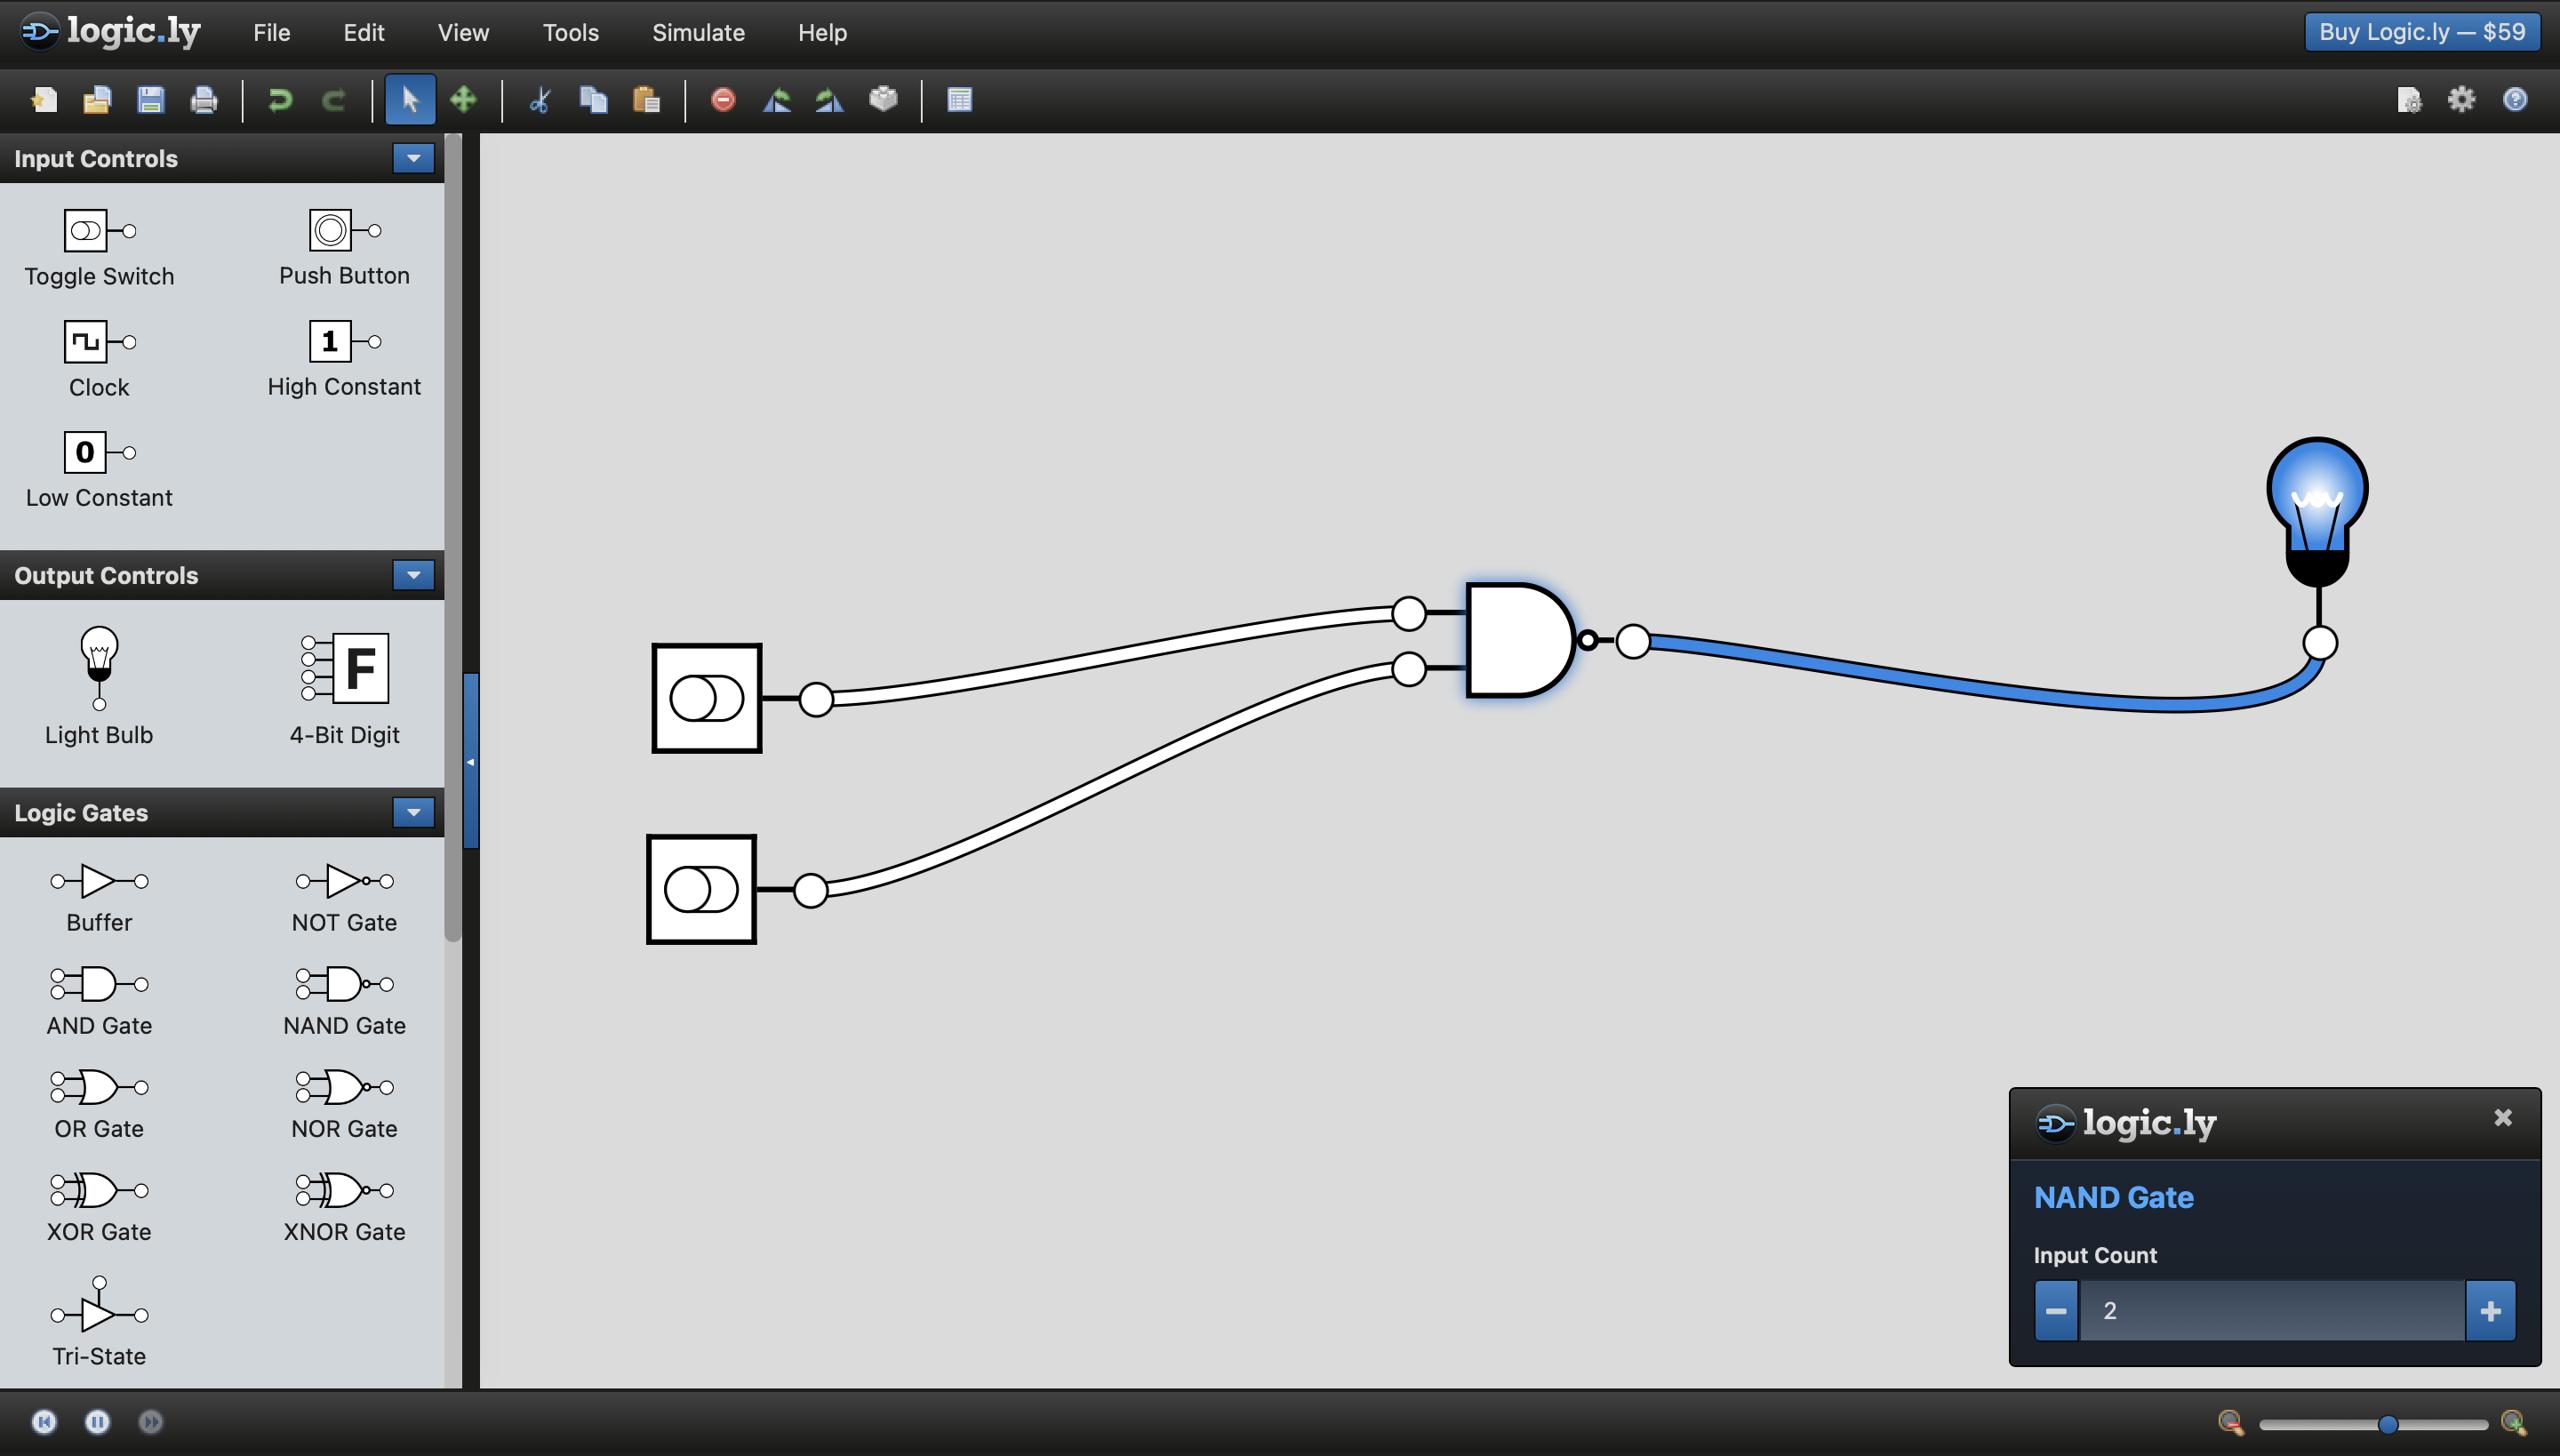
\includegraphics[width= 0.95\linewidth]{Zrzut ekranu 2025-01-25 o 22.20.30.png}\\ 
    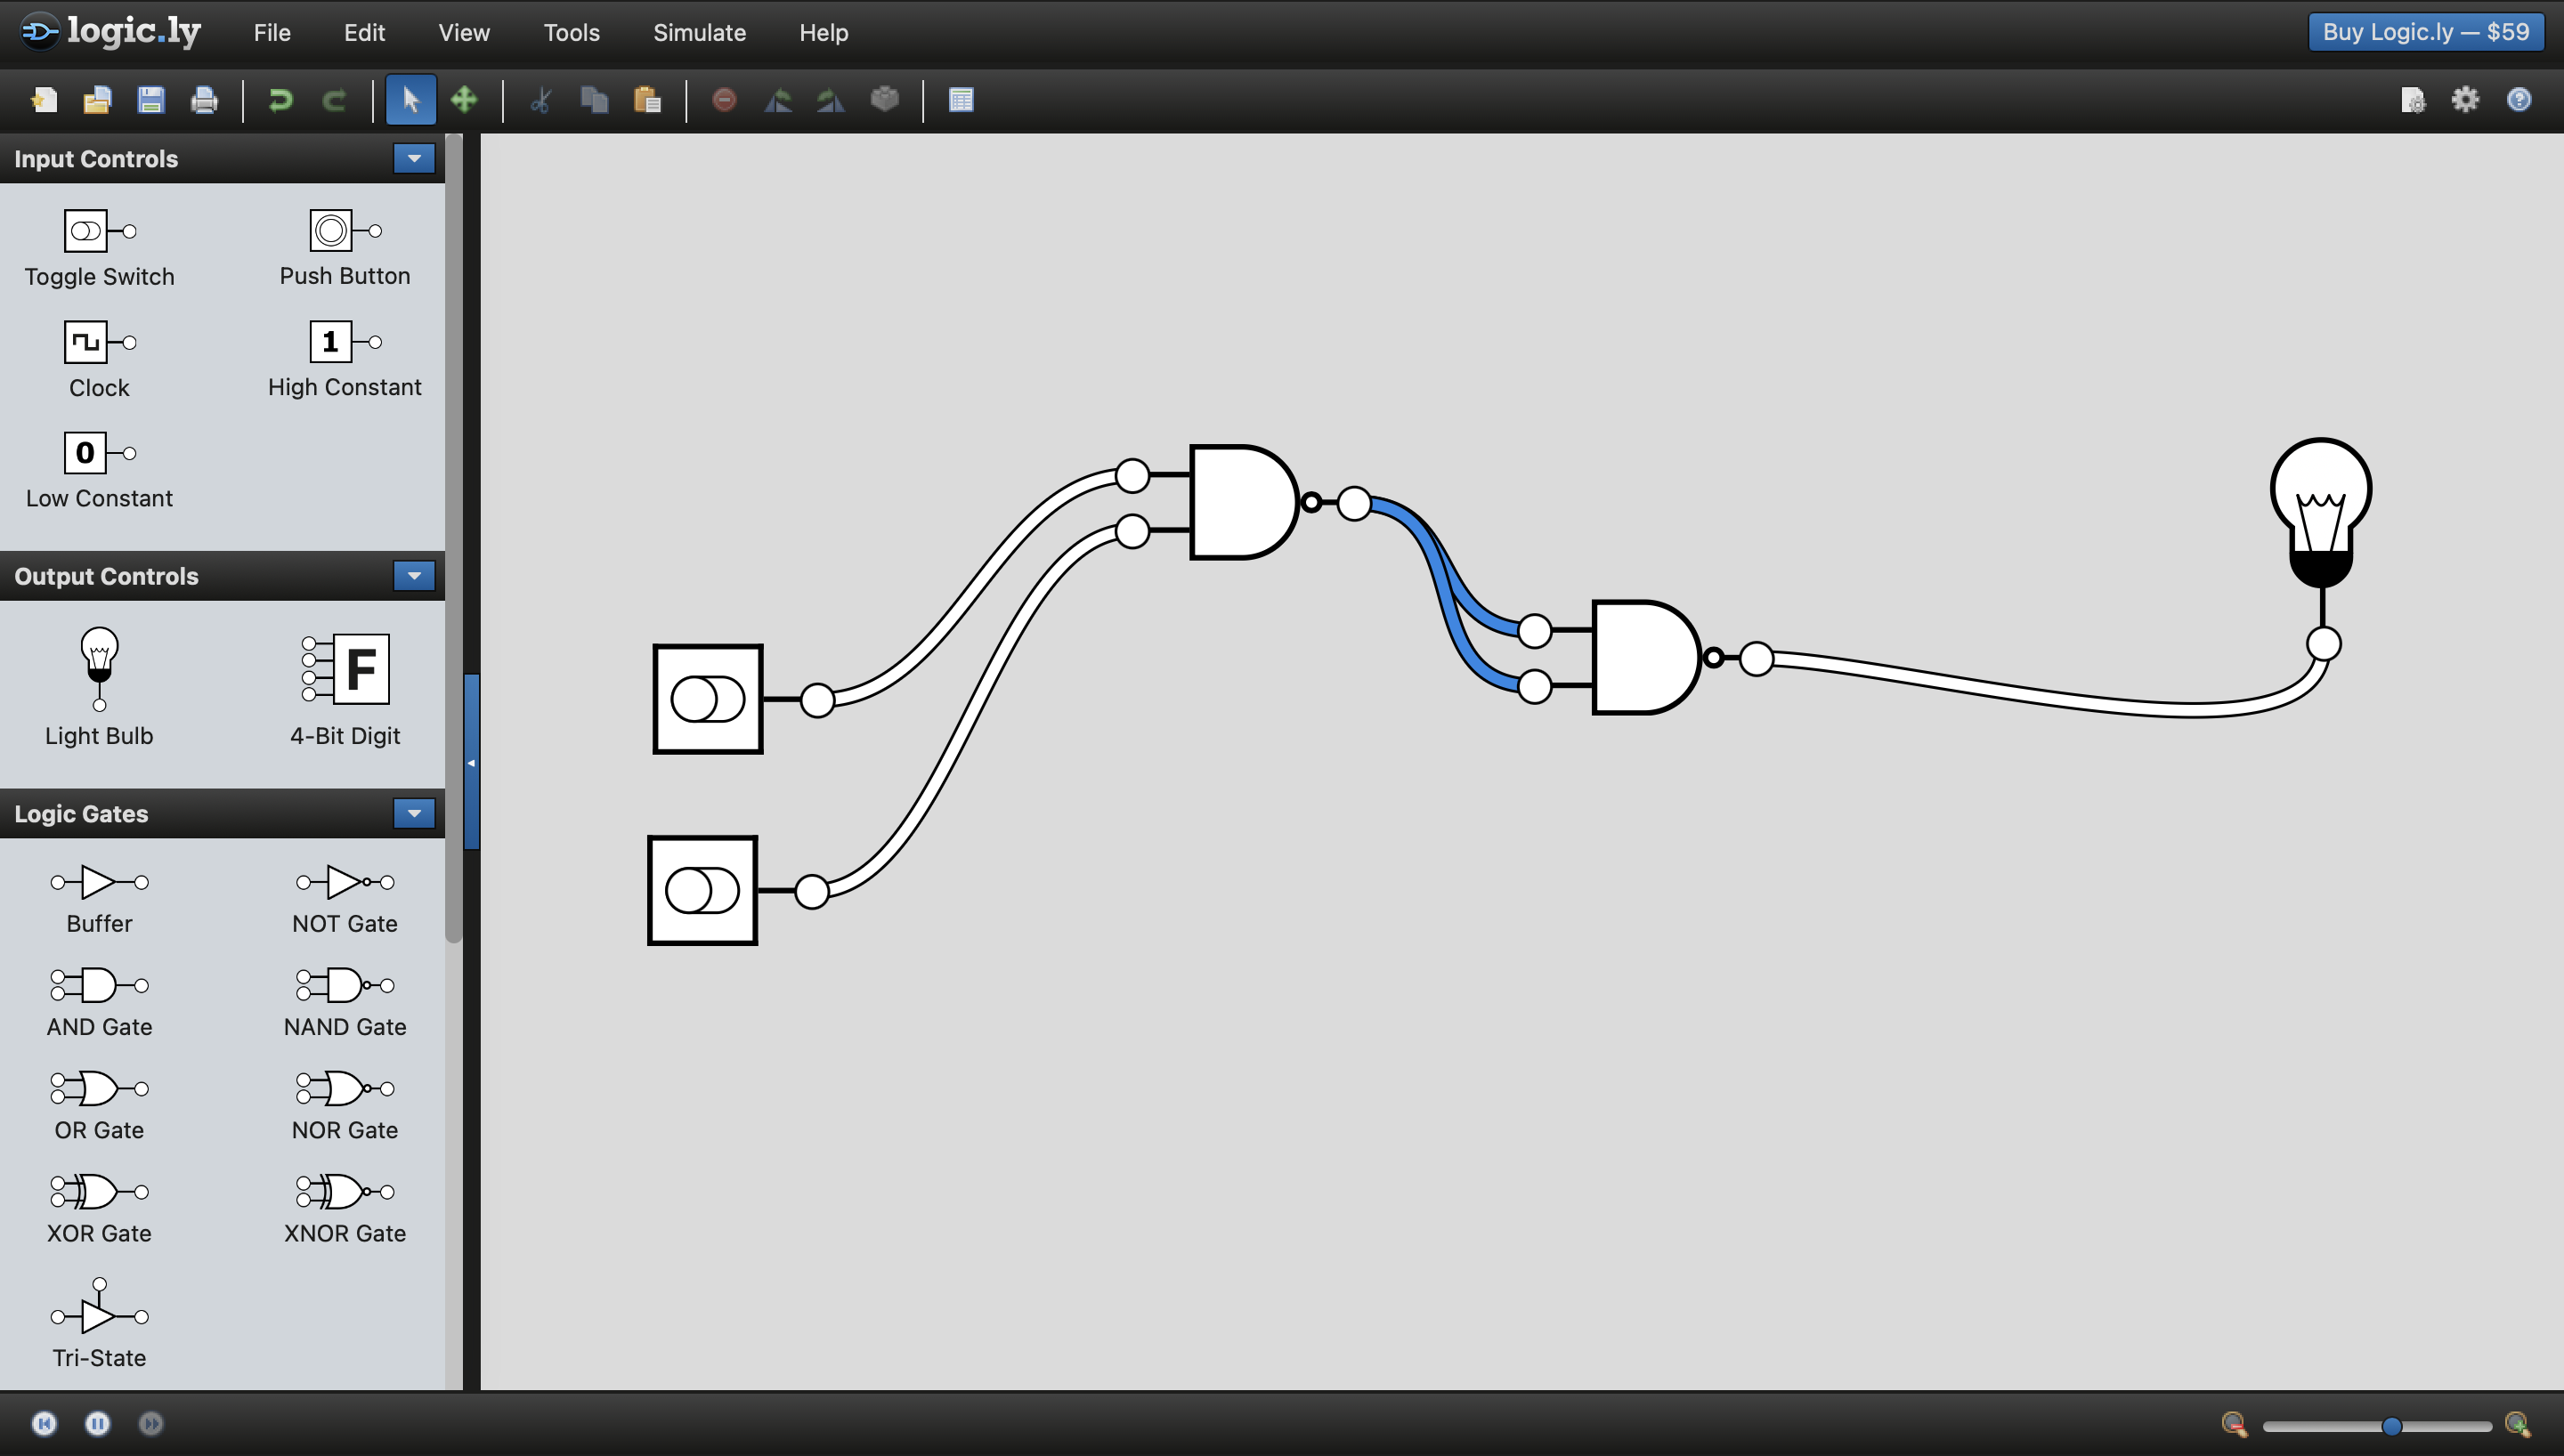
\includegraphics[width= 0.95\linewidth]{Zrzut ekranu 2025-01-25 o 22.20.16.png}\\
    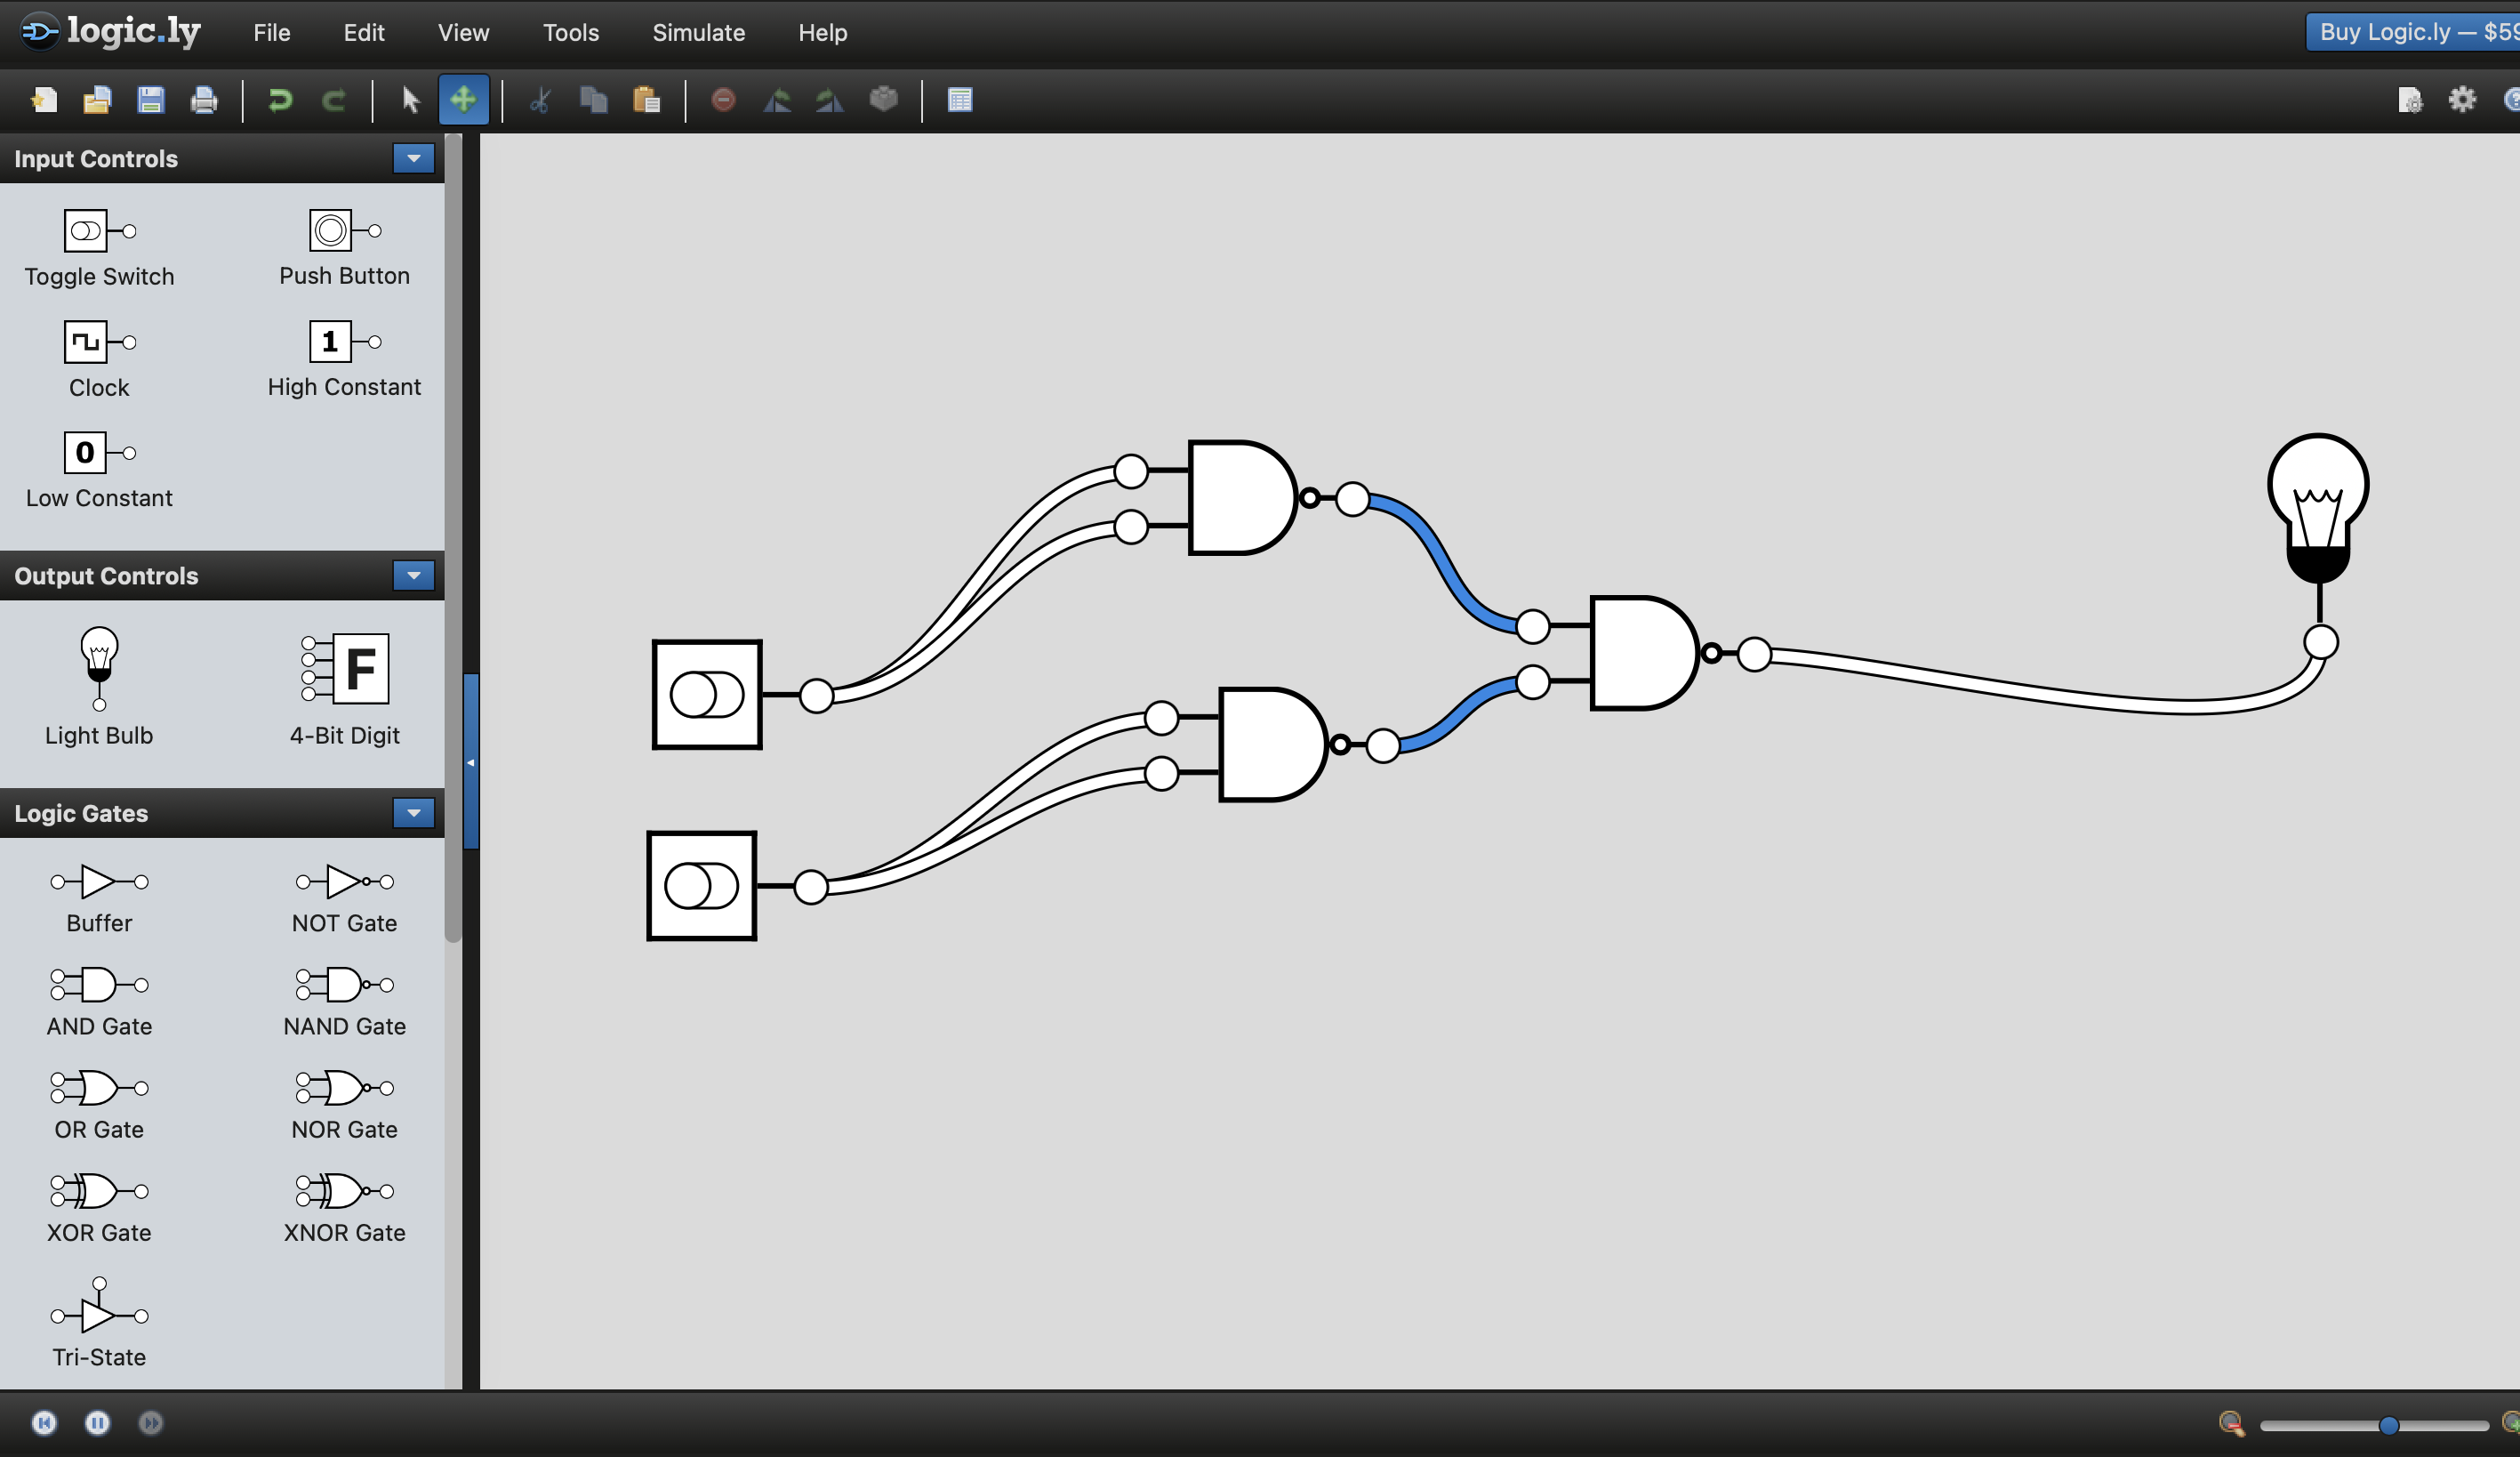
\includegraphics[width= 0.95\linewidth]{Zrzut ekranu 2025-01-25 o 22.19.33.png}
    
    

\end{document}
